

\chapter[辅助工作]{辅助工作}[Harbin Institute of Technology Postgraduate Dissertation Writing Specifications]

\section{相机选型与基本设置}[Content specification]

\subsection{引言}[Content specification]
相机是计算机视觉中非常重要的一部分,负责获取环境中的图像信息,为后续的图像处理和算法提供输入数据。
因此,在进行计算机视觉项目时,选择适合的相机和合理的设置相机参数设置是非常关键的。
本章根据RoboMaster比赛的赛场光照环境和检测算法要求选择合适的工业相机并给出具体的型号。

\subsection{相机选型策略}[Content specification]
尽量选择高帧率、感光片大的相机,在此基础上选择光圈大的镜头,焦距选择视情况而定。
下面详细阐述:\par

\begin{itemize}[itemindent=2em]
    \item 分辨率:一般分辨率越高,图像质量越好,越有利于识别算法和测距算法。但分辨率越高,图像最大采集帧率越低,
    且检测算法耗时增加,价格也相应越高。因此选择分辨率在30万到100万像素的相机即可。
    \item 帧率:帧率越高,运动图像捕捉能力越好。由于我们需要检测高速移动或者旋转的目标,因此帧率越高越好。
    根据应用场景需要捕捉的运动速度和动态要求,选择适合的帧率,对于RoboMaster比赛场景来说,150fps+的帧率能够满足基本要求。
    \item 传感器尺寸和类型:CMOS和CCD是现代数字图像传感器的两种常见类型。
    CMOS传感器具有低功耗、低噪声、高帧率等优点,且质量更小,所以选择CMOS相机。
    \item CMOS传感器有两种快门方式,卷帘快门和全局快门。
    全局快门曝光时间更短,但噪声更大;卷帘快门可以达到更高的帧速,但当
    曝光时间较长或物体移动较快时产生果冻效应。
    为了适应RoboMaster比赛场景的需求,选择全局快门的相机。
    \item 工作温度和防护等级:根据应用环境和需求,选择适合的工作温度和防护等级。
    工业相机一般需要在恶劣环境下工作,如高温、灰尘等,所以防护等级要求较高。
    \item 软件支持:算法运行环境为Linux,
    工业相机的软件平台需要支持图像处理和数据分析等功能,
    通常需要与特定的软件开发工具包配合使用,且售后的技术支持和SDK软件包的是否适合二次开发也是选择的考量重点。

\end{itemize}


一张成像清晰、亮度均匀的图片非常有利于后续的图像处理算法,因此如何设置相机参数,以及如何预处理原始图像后都非常重要。
\subsection{相机硬件设置}[Content specification]
拿到相机后,基本设置如下:将光圈拧到最大;调整成像平面与光心的距离,使得5m成像最清晰;涂抹螺丝胶,防止相机在剧烈震动的情况下因螺丝松动而成像不清。之所以将光圈拧到最大,是为了在达到相同图像亮度的情况下获得更短的曝光时间,进而提高相机帧率。
\subsection{相机软件设置}[Content specification]
模拟增益调高,目的:一是在达到相同图像亮度的情况尽可能减少曝光时间从而提高取图帧率,
不过由于增益拉高后图像噪点也会增加,因此需要平衡; 
二是使得发光体在图像中更加明显,从而二值化阈值可以取到非常高,可以防止过曝给灯条的提取造成影响,
因为即使在过曝的情况下,光晕的灰度值与真正的发光体还是有较大的区别,通过高阈值筛选可以很好的提取灯条。

设置相机白平衡参数,使得成像色彩正常,
迈德威视相机的软件工具包提供了自动调节白平衡参数的功能,只需要将相机对准白色物体,
然后点击“白平衡”按钮即可。

\subsection{本节小结}[Content specification]
本章主要介绍了相机选型、硬件设置和软件设置等方面的知识。
在相机选型方面,需要考虑分辨率、帧率、传感器尺寸和类型、工作温度和防护等级、
以及软件支持等因素。在硬件设置方面,需要注意光圈的设置和成像平面与光心的距离等。
在软件设置方面,需要注意模拟增益的调整和颜色通道增益的选择等。
明确这些方面的知识,可以使相机的使用更加得心应手,也能够为后续的图像处理和算法提供更好的输入数据。
\par
最终选择迈德威视相机,型号为MV-SUA34GC。规格参数在附录2中。


\section{主从机时钟对齐}[Content specification]


\subsection{引言}[Content specification]
在工业自动化和嵌入式系统中,上位机和下位机之间的时间同步是非常重要的。通常,下位机的时间通常是由硬件时钟提供的,
而上位机的时间通常是由操作系统提供的。由于硬件时钟和操作系统时钟存在不同步的可能,
因此需要基于通信方法来同步它们的时间,比如NTP就是一种用于同步计算机时钟的协议。
\par

然而由于下位机目前不支持网络服务,
因此本章参考NTP同步时钟的思路,通过上下位机的CAN通信实现了双机时钟的统一,
巧妙地解决了网络服务不可达的问题。

\subsection{通信时延测量}[Content specification]
对于一固定的装甲板,晃动云台,则理论上解算的装甲板在惯性系下的坐标是不变的。
然而,由于通信时延、相机成像时间误差、计时精度、陀螺仪数据精度与系统偏差等因素,
不可能精确的获得的图像对应的陀螺仪数据。这里面影响因素最大的就是通信时延,因此通过调节通信时延量,
使得惯性系下的装甲板坐标晃动幅度最后,此时得到的通信时延量被认为是真实的通信时延。
\par
图\ref{delay}展示了在通信时延量在超前、滞后、大致准确时解算的装甲板在惯性下的坐标。
\begin{figure}[H]
    \centering
    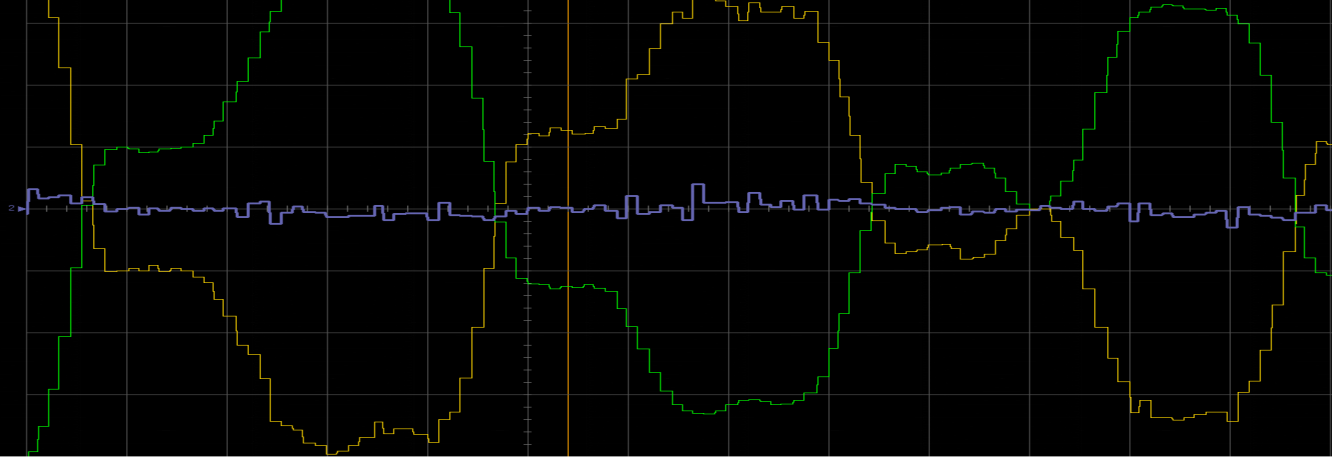
\includegraphics[width=.8\textwidth]{delay.png} 
    \caption{不同通信时延对应的装甲板惯性系下的坐标} 
    \label{delay}
\end{figure}

\subsection{动态时间帧对齐}[Content specification]

基本思想如下:事先通过上述技术手段测量通信时延。然后以下位机的时钟为基准,下位机定频(100$hz$)向上位机发送本机的时钟信息,上位机将计算本机时钟与下位机时钟之差(在考虑通信时延的情况下),
并将数据放入到循环队列中,当需要在上位机获取下位机时钟时刻时,
通过计算循环队列的平均值作为上下位机时钟偏移量加到本机时钟就可以获得下位机的时钟时刻,如图\ref{clock_sync}所示。

\begin{figure}[H]
    \centering
    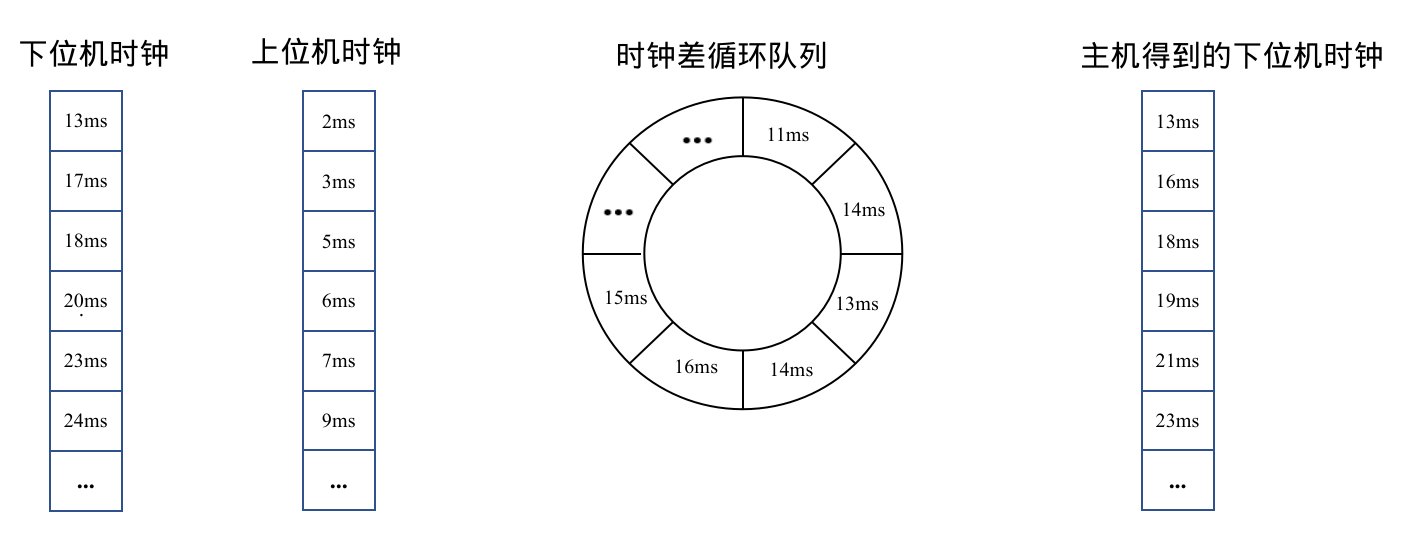
\includegraphics[width=.8\textwidth]{clock_sync.png} 
    \caption{自实现时钟同步} 
    \label{clock_sync}
\end{figure}

\subsection{本节小结}[Content specification]
通过观测固定装甲板惯性下的坐标浮动情况测量通信时延,基于通信实现动态上下位机时间帧对齐,
实现了双机时钟的统一,有利于后续的坐标转换、云台姿态控制等。


\section{受空气阻力的弹道迭代计算}[Content specification]


\subsection{引言}[Content specification]
在现代计算机计算中,迭代计算已经成为了一种非常重要的计算方法,
尤其是在物理学、工程学和计算机科学等领域中。
受空气阻力的影响,
弹道轨迹并不是一个简单的抛物线,
因此迭代计算成为了计算弹道轨迹的重要方法。


\subsection{空气阻力系数求解}[Content specification]
其中因为在y⽅向分速度较⼩,可以忽略不计,因此只考虑x⽅向的空⽓阻⼒。空气阻力计算公式如下:
\begin{gather}
    F = kv^2 =  \frac{1}{2} CS \rho  v^2
\end{gather}

\par

其中$\rho$为空气密度,一般取$1.293kg/m^3$,S为球截面积,$v$为球体速度,C为阻力系数,与雷诺数$R_e$有关系,关系如图\ref{空气阻力系数与雷诺数关系}所示。

\begin{figure}[H]
    \centering
    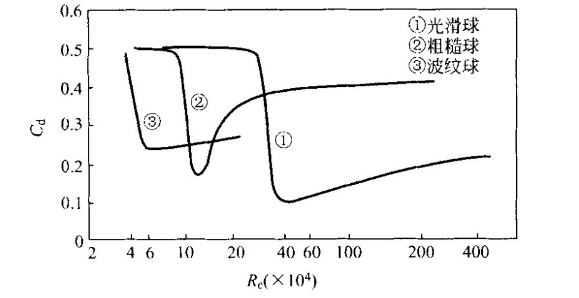
\includegraphics[width=.8\textwidth]{leinuo.png} 
    \caption{雷诺数} 
    \label{空气阻力系数与雷诺数关系}
\end{figure}

\par 

雷诺数计算公式如下:
\begin{gather}
    R_e = \frac{\rho v D}{\eta}
\end{gather}

其中$\rho$为空气密度,一般取$1.293kg/m^3$,D为物体直径,$v$为球体速度,$\eta$为空气粘滞系数,通常取$1.983\times10^{-5}pa\cdot s$


\subsection{弹道迭代计算}
\begin{figure}[H]
    \centering
    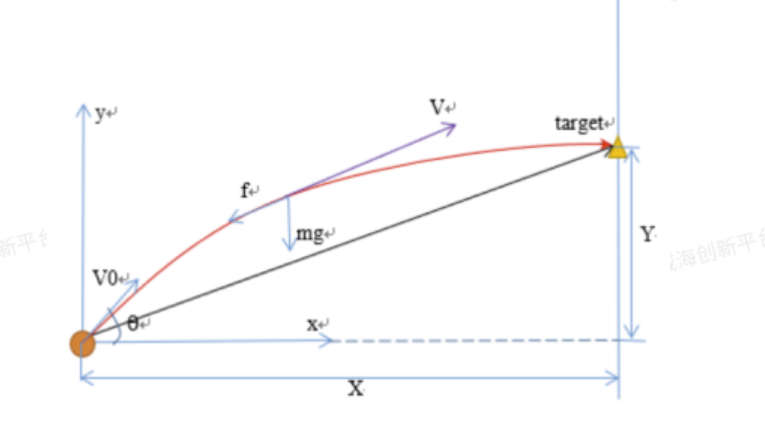
\includegraphics[width=.8\textwidth]{trajectory.png} 
    \caption{弹丸受力分析图} 
    \label{弹丸受力分析图}
\end{figure}

如上所述,我们只考虑水平方向的空气阻力。弹丸的动力学微分方程如下:
\begin{gather}
    m \frac{dv_x}{dt} = -k v_x^2 \\
    m \frac{dv_y}{dt} = -mg
\end{gather} 

采用分离变量法求解微分方程,可得:
\begin{gather}
    v_y = v_{y0}-gt \\
    v_x = \frac{m v_{x0}}{m+kv_{x0}t}
\end{gather}

消去时间变量$t$,可推导出如下动力学公式:
\begin{gather}
\frac{gm^2\lambda^2 tan^2(\theta)}{2k^2v^2}-\frac{\lambda m tan^2(\theta)}{k}+\frac{gm^2\lambda^2}{2k^2v^2}+y = 0
\end{gather}

其中:
\begin{gather}
    \lambda = e^{\frac{kx}{m}-1}
\end{gather}

代入目标位置即可求得子弹飞行时间$t$和云台姿态角$pitch$。\par
然而待击打的物体是在运动的,若是直接拿观测坐标计算弹道,则弹丸在打过去的时候,
目标已经离开原来位置,出现击打滞后现象。但是,考虑目标运动的弹道解算想要求解析解几乎是不可能的,因此我们退而求其次,通过数值
迭代的方式求数值解。基本思路为:
\begin{enumerate}
    \item 按照初始位置矢量计算弹道,解算飞行时间$t_0$。
    \item 根据此飞行时间计算目标位移量$\Delta \vec{x_0}$。
    \item 根据目标位移量计算新的位置矢量$\vec{x_1}$。
    \item 跳转至1过程。
\end{enumerate}

经过多次迭代之后即可收敛。收敛的判断条件可以设置为目标位移量低于一定阈值。

如图\ref{迭代计算过程}所示:

\begin{figure}[H]
    \centering
    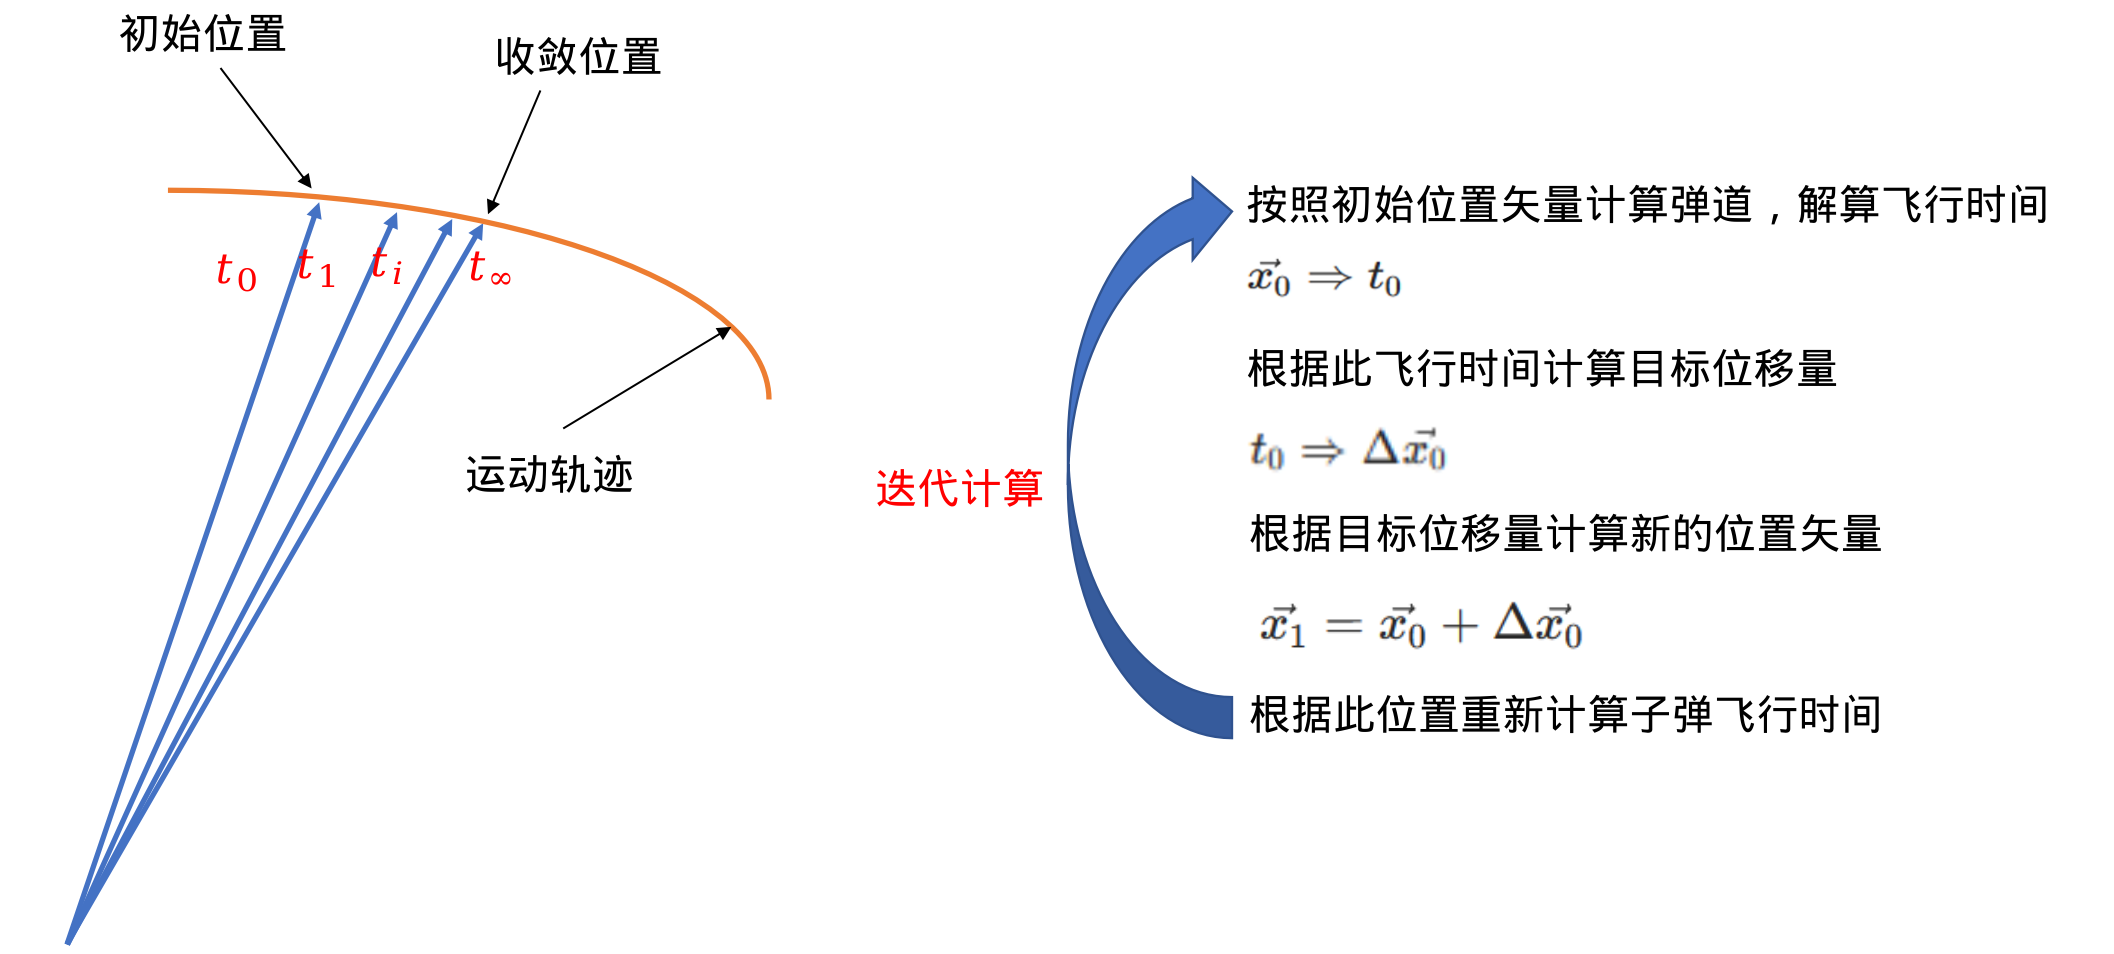
\includegraphics[width=.8\textwidth]{iter.png} 
    \caption{迭代计算过程} 
    \label{迭代计算过程}
\end{figure}

\subsection{弹道轨迹可视化}[Content specification]
使用matplotlib将受空气阻力影响的弹道轨迹和不受空气阻力影响的弹道轨迹可视化。如图\ref{弹道对比}所示,
绿色曲线为不受空气阻力影响的弹道轨迹,红色曲线为受空气阻力影响的弹道轨迹。
\begin{figure}[H]
    \centering
    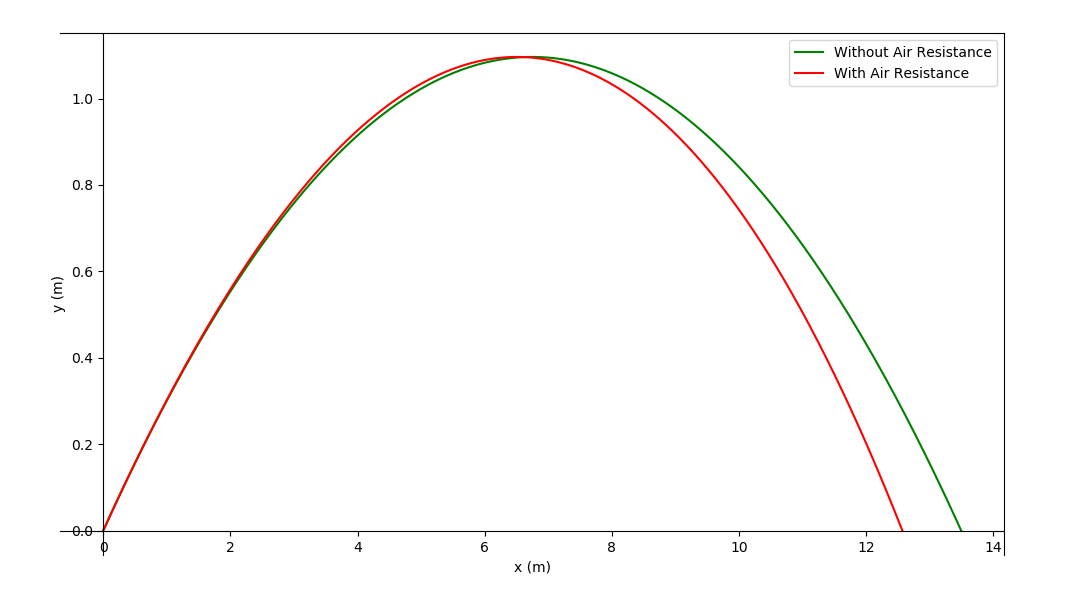
\includegraphics[width=.8\textwidth]{air_resistence_compare.png} 
    \caption{弹道对比图} 
    \label{弹道对比}
\end{figure}


\subsection{本节小结}[Content specification]
本章详细介绍了受空气阻力的弹道迭代计算方法,
包括空气阻力系数的求解和弹丸动力学微分方程的解析解。
针对目标运动情况,提出了数值迭代的解算方法,并给出了迭代计算过程和收敛条件。
最后将受空气阻力与不受空气阻力的弹道轨迹使用matplotlib可视化。
本文提供了一种可行的数值解决方案,对于弹道计算和精确打击目标具有重要意义。







